\documentclass[conference]{IEEEtran}
\IEEEoverridecommandlockouts
% The preceding line is only needed to identify funding in the first footnote. If that is unneeded, please comment it out.
\usepackage{cite}
\usepackage{amsmath,amssymb,amsfonts}
\usepackage{algorithmic}
\usepackage{graphicx}
\usepackage{textcomp}
\usepackage{xcolor}
\def\BibTeX{{\rm B\kern-.05em{\sc i\kern-.025em b}\kern-.08em
    T\kern-.1667em\lower.7ex\hbox{E}\kern-.125emX}}
\begin{document}

\title{Automated Network Packet Generation for Evaluation of Neural Networks in Intrusion Prevention Systems}

\author{\IEEEauthorblockN{Bernhard Gally}
\IEEEauthorblockA{\textit{IT Security} \\
\textit{FH Technikum Wien}\\
Vienna, Austria\\
cs19m023@technikum-wien.at}
\and
\IEEEauthorblockN{Sebastian Lipp}
\IEEEauthorblockA{\textit{IT Security} \\
\textit{FH Technikum Wien}\\
Vienna, Austria \\
cs19m032@technikum-wien.at}
\and
\IEEEauthorblockN{Damir Marijanovic}
\IEEEauthorblockA{\textit{IT Security} \\
\textit{FH Technikum Wien}\\
Vienna, Austria \\
cs19m031@technikum-wien.at}
}

\maketitle

\begin{abstract}
This Paper is a part of a project. It describes the part of automated network packet generation. The generated packets are used to evaluate neural networks in intrusion prevention systems. The challenges in this project include building the infrastructure and connecting the individual nodes in the network.
\end{abstract}

\begin{IEEEkeywords}
artificial intelligence, neural networks, computer networks, network security, packet generation
\end{IEEEkeywords}

\section{Introduction}
For a good, respectively successful detection of malicious network traffic using neural networks, the neural network has to be trained well. Therefore a large set of labelled network traffic is necessary. The more attack scenarios there were, the better the differentiation between attacks and normal traffic. Of course, not all possible scenarios can be dealt with here, which is why you have to concentrate on the attacks that occur most often in the real world. This subproject relates to the generation, labelling, distribution and recording of network data and packets. The network was deliberately kept simple and the different types of attacks were treated separately. The infrastructure was considered from scratch and implemented into a network simulation tool called \textit{GNS3}. To make the individual parts dynamic, the decision was made to use docker containers. This made it possible to evaluate the individual scenarios separately. The traffic was recorded using the \textit{tcpdump}, and the entire filtered traffic was saved in so-called pcap files. As far as the hardware is concerned, sufficient computing power was required, as well as sufficient storage space to be able to record the traffic. 


\section{Infrastructure}

This chapter covers the design of an infrastructure which provides a tool for creating generic environments in which specific network scenarios can be simulated to record network packets and extract features with which neural networks inside intrusion prevention systems could be trained and evaluated.

This work is split into four parts. The first part designs the fundamental simulation architecture. The second focuses on the creation of network nodes, followed by the configuration of the network in the third part. The last part covers the automation of the procedure with the help of provioning tools.

\subsection{Designing the architecture}

A simulation network consists of multiple scenarios based on network attacks and benign traffic. In this network, generic hosts can be placed and connected to each other or the internet with the usage of hubs, switches and routers. These hosts reflect attackers and victims or usual clients and servers, as well as recorders. To ensure recorded features can be labeled, recorders are placed on all positions where another kind of attack or network traffic should be recorded. Furthermore, they are able to filter out selected traffic to ensure only the important traffic is recorded. This means network traffic is recorded within multiple files marked as bad or good which serve as input for the data extractor to extract the features and create the dataset to train and test the neural network.

\begin{figure}[htbp]
\centerline{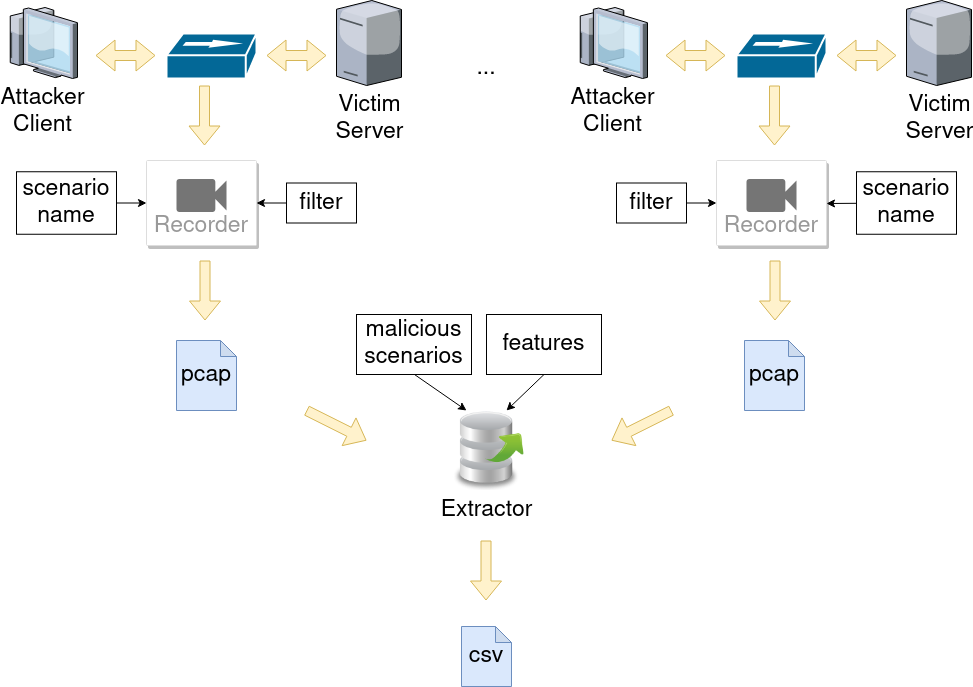
\includegraphics[scale=0.26]{principle.png}}
\caption{Design principle}
\label{principle}
\end{figure}

Fig.~\ref{principle} shows the design principle. The recorders receive the data through network hubs placed between the attackers and victims or clients and servers and record in pcap files to a central filesystem. The scenario names and filter settings are passed to the recorders as parameters. The recorded files - named after the associated scenario - are then collected and forwarded to the extractor which knows the names of the malicious scenarios and extracts the selected features to a csv file. The extractor is only required once and is not part of the simulation environment. 

\newpage 

\subsection{Creating the nodes}

\begin{figure}[htbp]
\centerline{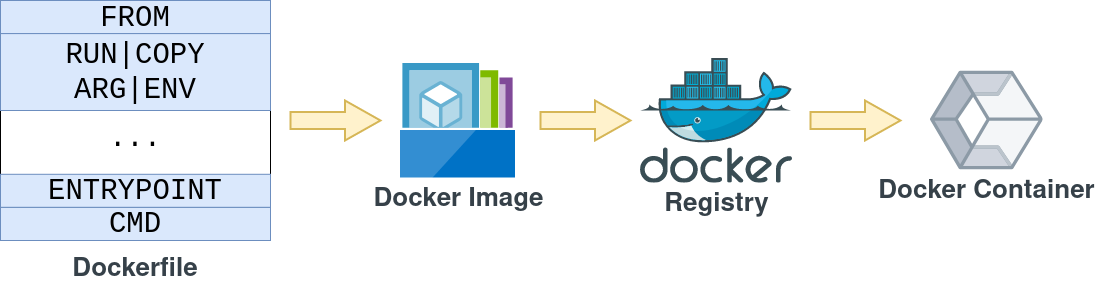
\includegraphics[scale=0.24]{docker.png}}
\caption{Node creation}
\label{node_creation}
\end{figure}

Docker containers are used for creating customized network nodes to offer users a very generic approach. The configuration of the nodes is based on code and can be easily created. It is defined within Dockerfiles which can be transformed to an image and uploaded to a registry through Docker client tools as shown in Fig.~\ref{node_creation}. When the images are placed on a public Docker registry, they can be pulled and executed from anywhere. This is the default approach in the current infrastructure design. 

The lines in a Dockerfile describe the layers of which the image consists. The first line is a statement to specify the base image, for example Alpine Linux or Ubuntu. The new image inherites everything from this base layer. After that, multiple commands can be added to install software, configure the system, copy files to the image or define environment variables. The last lines define the entrypoint and/or a command which the container runs when it is started. This could be for instance a program to attack a host or record the network traffic. Docker also supports mounting volumes to the containers when they are started as well as passing arguments to use the same image for similar nodes with different settings. More about creating Dockerfiles can be found on the offical documentation of Docker.\footnote{https://docs.docker.com/develop/develop-images/dockerfile\_best-practices} 

Once the images are built and uploaded to an accessible registry, they can be further used in the simulation environment. The target hosts only need the Docker runtime environment installed and access to the image registry. In this case the official Docker Hub is used to build and store the images for the scenarios. This includes all clients, servers, the recorder and the extractor.

The network recorder is based on a customized Docker image which runs tcpdump with additional arguments like the filename to specify the scenario name and the filter expression to sort out unwanted traffic. It records the packets passing the first interface. For more information about possible commands and configuration refer to the manpage of tcpdump.\footnote{https://www.tcpdump.org/manpages/tcpdump.1.html}

The extractor, or more precisely the CI flowmeter, is also placed into a Docker container mounting a volume containing all the recorded pcap files. It extracts only the features defined by a parameter and saves the csv file with the extracted features at the same place as the pcap files, which can be later transferred to another host to evaluate the data.

The runtime configuration and connection of the network nodes as well as the creation of other nodes like switches, hubs and routers is part of the simulation environment which is covered in the next section.

\subsection{Connecting the nodes}

The configuration of the network, or more precisely the connection between the network nodes, is done within GNS3, an open-source network simulator which can be easily controlled via a native graphical user interface or RESTful API. It consists of a server and a client application. In this setup, the server application is installed on a virtual machine which offers 8-cores, 32 GiB RAM and 300 GiB hard disk space. It is possible to install multiple servers, but in this case one was sufficient for simulating multiple scenarios including DoS attacks. More information about the installation of the server can be found on the official website of the GNS3 project.\footnote{https://docs.gns3.com/1c2Iyiczy6efnv-TS\_4Hc7p11gn03-ytz9ukgwFfckDk/index.html} 

Once the server runs, a project can be created and the scenarios can be configured via the graphical interface of the GNS3 GUI. It is recommended to setup a VPN to the server to ensure the terminals of the network nodes are reachable remotely without configuring network tunnels. This means it is necessary to connect to the server via VPN before the GUI can reach the server applicaiton.

\begin{figure}[htbp]
\centerline{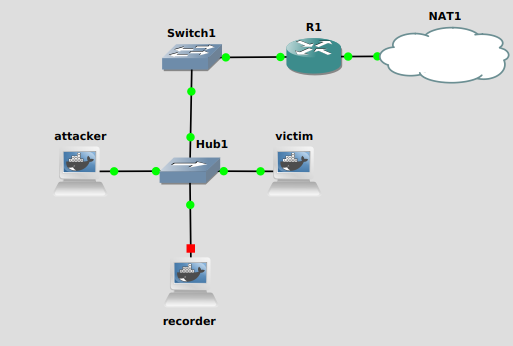
\includegraphics[scale=0.5]{network.png}}
\caption{Network example}
\label{network}
\end{figure}

Fig.~\ref{network} shows a simple network created in GNS3. The attacker, victim and recorder are created through Docker templates referring to the prevously created Docker images. GNS3 supports the configuration of environment variables and volumes for Docker containers. All other components, including switches, routers and the interface to the internet, are basic network components of GNS3 and are already available in the device browser. Cisco routers need official IOS images before they can be created.

The project is automatically saved to the filesystem and includes all components which are needed to run the network, including configuration, logs and recorded data. The simulation can be started through the GUI or the API and produces the pcap files within the project directory. Once the simulation is stopped, the pcap files can be copied to a temporary directory and sent through the extractor container to produce the csv file including the extracted features.

\begin{figure}[htbp]
\centerline{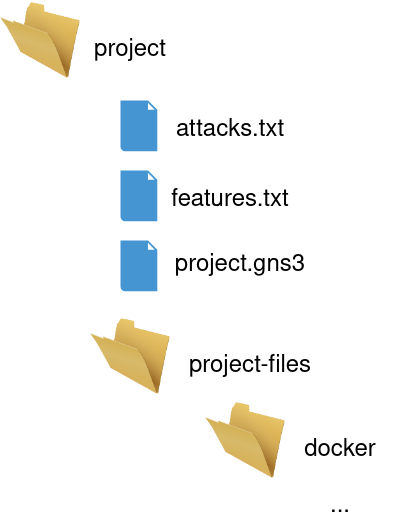
\includegraphics[scale=0.33]{project.png}}
\caption{Project structure}
\label{project}
\end{figure}

The setup of the network is done through the GUI because the API does not support all features to create network nodes. The project folder can be checked into version control and copied to the server when it is needed. As shown in Fig.~\ref{project}, it consists of the gns3 file which contains all the network configuration in a JSON format. The project-files directory contains additional files which are part of the filesystems of the network nodes, for example the docker containers. The text files are the parameters, which are passed to the extractor to determine the attack names and the features to extract.

\subsection{Automating the procedure}

The automated setup of the server and run of the simulation is done within Anisble playbooks. Therefore, multiple roles are created, one for the setup of the GNS3 server, one for running the network simulation and one for extracting the features. As shown in Fig.~\ref{ansible}, the server role is associated with the setup playbook, while the simulation and extraction roles are used by the run playbook. These playbooks are stored in YAMl files and can be executed with the ansible tools.\footnote{https://docs.ansible.com/ansible/latest/user\_guide/playbooks.html\#working-with-playbooks}  

\begin{figure}[htbp]
\centerline{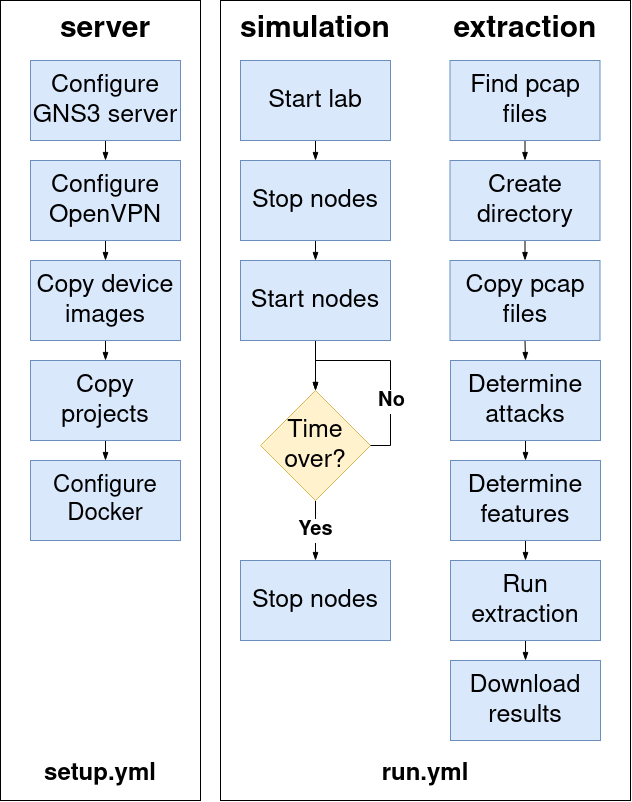
\includegraphics[scale=0.33]{ansible.png}}
\caption{Ansible roles}
\label{ansible}
\end{figure}

The server role sets up the GNS3 server and OpenVPN, copies the device images and projects and configures the Docker runtime environment. It downloads the VPN configuration to the client, which can be later used to connect to the server. Because the test setup restricted the incoming ports, VPN was changed to use TCP instead of UDP to enable the functionality of creating SSH tunnels.

To run the simulation role, a VPN connection to the server is required. This is accomplished by a simple connection script which opens an SSH tunnel and connects to the server via VPN. This is necessary because Ansible needs access to the GNS3 API and the network components. When the role is executed, it opens the project and restarts all network nodes. The duration can be defined through a parameter. When the time is over, the nodes are stopped. To control GNS3 via the API, an additional Ansible collection is used. \footnote{https://github.com/davidban77/ansible-collection-gns3}

The extraction role gathers the pcap files, creates a temporary directory and copies all files there. Then it determines all attack scenarios and features from a file in the project directory and runs the extraction container with the mounted pcap volume and the passed parameters. After that it downloads the csv file with the extracted features. If specified in a parameter, the pcap files are also downloaded.

The server can be setup by running the following command:
\begin{verbatim}
ansible-playbook -i hosts setup.yml 
                 --ask-become-pass
\end{verbatim}

Once the GNS3 projects are checked into the Ansible project folder, the simulation can be started with the following command:
\begin{verbatim}
./connect.sh
ansible-playbook -i hosts run.yml
                 --ask-become-pass
                 -e project=<project_name>
                 -e duration=<minutes>
                 [-e pcap=true]
\end{verbatim}

All Ansible commands must be executed within the gns3 folder and need the sudo password from the server user. The hosts file contains the target hosts configuration.

The next chapter focuses on the implementation and simulation of specific scenarios within a GNS3 project with the help of the introduced infrastructure to produce a new dataset for evaluating neural networks in IPS systems.  

\section{Simulation}
@Bernhard [2-3p]

\section{Conclusion}
The result of this project can be used in the knowledge as well as in the structure. Due to the dynamic structure of the infrastructure, extensions can be added with little effort. During the implementation of the infrastructure, minor difficulties came up again and again, but these could usually be remedied with a relatively small change. Among other things, difficulties arose in the transfer of environment variables in the individual Docker containers. The other part of this project used this project as the basis, in which the recorded information and packages were evaluated. The successful evaluation showed that both the infrastructure and the individual nodes worked well.

\begin{thebibliography}{00}
\bibitem{b1} zzz
\end{thebibliography}

\end{document}
